%% main.tex — University of Piraeus Assignment Template
%% Compile with: pdflatex main.tex (run twice for TOC/references)
%%
\documentclass{unipi-assignment}

% ─── Additional packages ─────────────────────────────────────────────────
\usepackage{lipsum}        % Dummy text (remove in final document)
\usepackage{csquotes}      % Proper quoting

% ─── Document metadata ───────────────────────────────────────────────────
\doctitle{Scientific Writing in Education}       % Header left
\docauthor{Student Name}                         % Header right

% Title page fields
\university{UNIVERSITY OF PIRAEUS}
\school{SCHOOL OF INFORMATION AND COMMUNICATION TECHNOLOGIES}
\department{DEPARTMENT OF INFORMATICS}
\coursetitle{Course Assignment}
\coursename{Scientific Writing in Education}
\essaytitle{}
\studentname{}
\fathername{}
\studentid{P/XXXXX}
\submissiondate{Month Year}

% ═════════════════════════════════════════════════════════════════════════
\begin{document}

% ─── Title Page (no header/footer, no page number) ──────────────────────
\maketitlepage

% ─── Front Matter (roman numerals start at copyright) ───────────────────
\frontmatter

% ─── Copyright Page (header + footer, roman numerals) ───────────────────
\makecopyrightpage

% --- Abstract ---
% --- Abstract ---
\sectionunnumbered{Abstract}

\begin{indented}
  % Write your abstract here. The abstract should summarize the main
  % objectives, methods, results, and conclusions of the paper in a
  % concise manner. It typically ranges from 150 to 300 words.
\end{indented}

\vspace{160pt}
{\itshape\color{heading1color}Keywords:\/} keyword1, keyword2, keyword3

\clearpage
\hbox{}%
\clearpage


% --- Table of Contents ---
\tableofcontents

\clearpage

% --- List of Figures ---
\listoffigures

\clearpage

% --- List of Tables ---
\listoftables

\clearpage

% --- List of Diagrams ---
\listofdiagrams

\clearpage

% ─── Main Matter (arabic numerals, starting from 1) ────────────────────
\mainmatter

% --- Introduction ---
% --- Introduction ---
\sectionunnumbered{Introduction}

Recommended reference citation formats:

\begin{indented}
  \begin{itemize}
    \item Journals: See reference~\cite{wu2004}
    \item Books and monographs: See reference~\cite{levenspiel2002}   
    \item Conference proceedings: See reference~\cite{bock1984}\
    \item Multi-author texts: See reference~\cite{deuflhard1987}  
  \end{itemize}  
\end{indented}


% ═══════════════════════════════════════════════════════════════════════
% CHAPTER 1
% ═══════════════════════════════════════════════════════════════════════
% ═══════════════════════════════════════════════════════════════════════
% CHAPTER 1
% ═══════════════════════════════════════════════════════════════════════
\section{Chapter Title}

\bigskip

\subsection{Subchapter Title}

\bigskip

\subsubsection{Title \ldots}

\bigskip

% Example: figure within text
\begin{figure}[htbp]
  \centering
  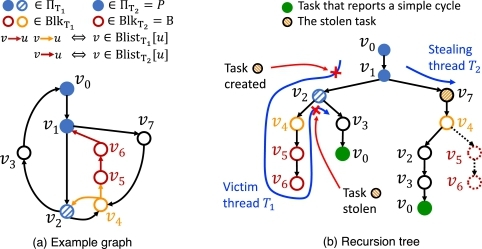
\includegraphics[width=0.7\textwidth]{images/figure-1.1.jpg}
  \caption{Description of the first figure of the first chapter.}
  \label{fig:1.1}
\end{figure}

\subsubsection{Title \ldots}

\bigskip

\subsubsection{Title \ldots}

\bigskip

% Example: figure within text
\begin{figure}[htbp]
  \centering
  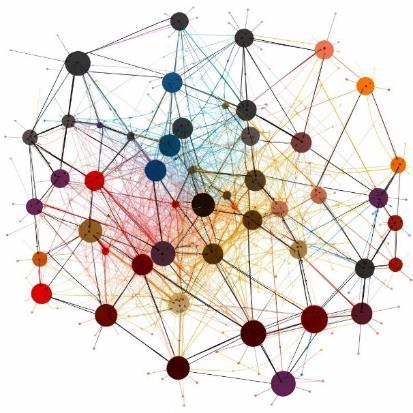
\includegraphics[width=0.5\textwidth]{images/figure-1.2.jpg}
  \caption{Description of the second figure of the first chapter.}
  \label{fig:1.2}
\end{figure}
\subsection{Subchapter Title}

\bigskip

\begin{indented}
  % Body text with indentation goes here
\end{indented}

\subsubsection{Title \ldots}

\bigskip

\subsubsection{Title \ldots}

\bigskip

\subsubsection{Title \ldots}

\bigskip
\subsection{Subchapter Title}

\bigskip

\subsubsection{Title \ldots}

\bigskip

\subsubsection{Title \ldots}

\bigskip

\subsubsection{Title \ldots}

\bigskip


% ═══════════════════════════════════════════════════════════════════════
% CHAPTER 2
% ═══════════════════════════════════════════════════════════════════════
% ═══════════════════════════════════════════════════════════════════════
% CHAPTER 2
% ═══════════════════════════════════════════════════════════════════════
\section{Chapter Title}

\bigskip

\subsection{Subchapter Title}

\bigskip

\subsubsection{Title \ldots}

\bigskip

\subsubsection{Title \ldots}

\bigskip

% Example: figure within text
\begin{figure}[htbp]
  \centering
  
\includegraphics[width=0.7\textwidth]{images/figure-2.1.jpg}
  \caption{Description of the first figure of the second chapter.}
  \label{fig:2.1}
\end{figure}

\subsubsection{Title \ldots}

\bigskip

\subsection{Subchapter Title}

\bigskip

\subsubsection{Title \ldots}

\bigskip

\subsubsection{Title \ldots}

\bigskip

\subsubsection{Title \ldots}

\bigskip
\subsection{Subchapter Title}

\bigskip

\subsubsection{Title \ldots}

\bigskip

\subsubsection{Title \ldots}

\bigskip

\subsubsection{Title \ldots}

\bigskip



% ═══════════════════════════════════════════════════════════════════════
% CHAPTER 3
% ═══════════════════════════════════════════════════════════════════════
% ═══════════════════════════════════════════════════════════════════════
% CHAPTER 3
% ═══════════════════════════════════════════════════════════════════════
\section{Chapter Title}

\bigskip

\subsection{Subchapter Title}

\bigskip

\subsubsection{Title \ldots}

\bigskip

\subsubsection{Title \ldots}

\bigskip

\subsubsection{Title \ldots}

\bigskip

\subsection{Subchapter Title}

\bigskip

\subsubsection{Title \ldots}

\bigskip

\subsubsection{Title \ldots}

\bigskip

\subsubsection{Title \ldots}

\bigskip

% Example: figure
\begin{figure}[htbp]
  \centering
  
\includegraphics[width=0.7\textwidth]{images/figure-3.1.jpg}
  \caption{Description of the first figure of the third chapter.}
  \label{fig:3.1}
\end{figure}

\subsection{Subchapter Title}

\bigskip

\subsubsection{Title \ldots}

\bigskip

\subsubsection{Title \ldots}

\bigskip

\subsubsection{Title \ldots}

\bigskip



% ═══════════════════════════════════════════════════════════════════════
% CHAPTER 4
% ═══════════════════════════════════════════════════════════════════════
% ═══════════════════════════════════════════════════════════════════════
% CHAPTER 4
% ═══════════════════════════════════════════════════════════════════════
\section{Chapter Title}

\bigskip

\subsection{Subchapter Title}

\bigskip

\subsubsection{Title \ldots}

\bigskip

\subsubsection{Title \ldots}

\bigskip

\subsubsection{Title \ldots}

\bigskip

\subsection{Subchapter Title}

\bigskip

\subsubsection{Title \ldots}

\bigskip

% Example: diagram (custom float)
\begin{diagram}[htbp]
  \centering
  
\includegraphics[width=0.7\textwidth]{images/diagram-4.1.jpg}
  \caption{First diagram}
  \label{diag:4.1}
\end{diagram}

\subsubsection{Title \ldots}

\bigskip

% Example: data table
\begin{table}[htbp]
  \centering
  \caption{First table}
  \label{tab:4.1}
  \begin{tabular}{lccc}
    \toprule
    \textbf{Type} & \textbf{Value 1} & \textbf{Value 2} & \textbf{Value 3} \\
    \midrule
    A & 0.93 & 1.28 & 2.47 \\
    B & 0.82 & 1.39 & 2.89 \\
    C & 0.75 & 1.32 & 3.14 \\
    \bottomrule
  \end{tabular}
\end{table}

\subsubsection{Title \ldots}

\bigskip

\begin{indented}
  % Body text with indentation
\end{indented}

\subsection{Subchapter Title}

\bigskip

\subsubsection{Title \ldots}

\bigskip

\subsubsection{Title \ldots}

\bigskip

% Example: second diagram
\begin{diagram}[H]
  \centering
  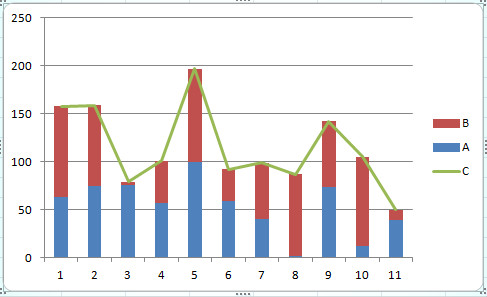
\includegraphics[width=0.7\textwidth]{images/diagram-4.2.jpg}
  \caption{Second diagram}
  \label{diag:4.2}
\end{diagram}

\subsubsection{Title \ldots}

\bigskip

% Example: second data table
\begin{table}[H]
  \centering
  \caption{Second table}
  \label{tab:4.2}
  \begin{tabular}{lccc}
    \toprule
    \textbf{Type} & \textbf{Value 1} & \textbf{Value 2} & \textbf{Value 3} \\
    \midrule
    A & 0.93 & 1.28 & 2.47 \\
    B & 0.82 & 1.39 & 2.89 \\
    C & 0.75 & 1.32 & 3.14 \\
    \bottomrule
  \end{tabular}
\end{table}



% ═══════════════════════════════════════════════════════════════════════
% CONCLUSIONS (unnumbered)
% ═══════════════════════════════════════════════════════════════════════
% ═══════════════════════════════════════════════════════════════════════
% CONCLUSIONS (unnumbered)
% ═══════════════════════════════════════════════════════════════════════
\sectionunnumbered{Conclusions}

% Write your conclusions here.


% ═══════════════════════════════════════════════════════════════════════
% BIBLIOGRAPHY (unnumbered)
% ═══════════════════════════════════════════════════════════════════════
\bibliographystyle{unsrt}
\bibliography{references}

% ═══════════════════════════════════════════════════════════════════════
% APPENDICES (unnumbered section header, then lettered appendices)
% ═══════════════════════════════════════════════════════════════════════
% ═══════════════════════════════════════════════════════════════════════
% APPENDICES (unnumbered section header, then lettered appendices)
% ═══════════════════════════════════════════════════════════════════════
\sectionunnumbered{Appendices}

\newpage

\makeappendixheading{}

% Content of Appendix A


\newpage

\makeappendixheading{}

% Content of Appendix B


\newpage


\end{document}
